\documentclass{acm_proc_article-sp}
\makeatletter
\def\@copyrightspace{\relax}
\makeatother

\usepackage{graphicx}
\usepackage{url}
\usepackage{eurosym}

\begin{document}

% 1. Report title, authors, and support cast (Lab assistant and course instructors). For each person, give name and contact information (email).
\title{GaussianCloud}
\subtitle{A cloud-based image blurring application}

\numberofauthors{5}
\author{
\alignauthor
R.M. de Lange\\
		\affaddr{1534068}\\
		\email{\{r.m.delange,}
\alignauthor
M. Voinea\\
		\affaddr{4317602}\\
		\email{m.voinea\}@student.tudelft.nl}
\and
\alignauthor
D.H.J. Epema\\
		\affaddr{Course Instructor}\\
		\email{\{d.h.j.epema,}
\alignauthor
A. Iosup\\
		\affaddr{Course Instructor}\\
		\email{a.iosup,}
\alignauthor
B.I. Ghit\\
		\affaddr{Lab Assistant}\\
		\email{b.i.ghit\}@tudelft.nl}
}

\maketitle

% 2. Abstract: a description of the problem, system description, analysis overview, and one main result. Size: one paragraph with at most 150 words.
\begin{abstract}
\end{abstract}

% 3. Introduction (recommended size, including points 1 and 2: 1 page): describe the
% problem, the existing systems and/or tools (related work), the system you are about to
% implement, and the structure of the remainder of the article; use one short paragraph
% for each.
\section{Introduction}
\label{sec:intro}
WantCloud BV is an organisation with a large workload in blurring images.
One of the business processes in WantCloud requires large images to be blurred using a Gaussian blur.
This process is compute intensive, as Gaussian functions require complex calculations as well as reading and writing large amounts of data.

Currently, WantCloud has a single server running all of these tasks.
For applying the Gaussian blur, an image filtering implementation in Java by Jerry Huxtable is used.\cite{web:huxtable}
The WantCloud server is experiencing heavy peak loads and sits idle for the rest of the day.
At peak moments clients need to wait for quite some time for the images to be processed, which is harmful for WantCloud's business.
Therefore, WantCloud wants to explore the option to utilise a cloud computing infrastructure to cope with high loads and be able to scale down with low loads.

This report will discuss the details of an exploration towards using Amazon EC2\cite{web:ec2} as a solution to WantClouds needs.
The image processing system will be implemented on a dynamically scalable cluster of compute nodes.
This implementation is made available open source through GitHub\cite{web:git}.
The performance, overhead, and scalability will be tested to compare to the current set-up using one machine.

In this report first an insight will be given into the background of the application and its requirements in Section \ref{sec:bg}.
After this the design of the cloud solution will be discussed in Section \ref{sec:system}, giving an insight in the implementation.
The designed system will be tested and evaluated in Section \ref{sec:eval}.
The results of the evaluation will be discussed in Section \ref{sec:discussion} and conclusions will be presented in Section \ref{sec:conclusion}.

% 4. Background on Application (recommended size: 0.5 pages):
% describe the application (1 paragraph) and its requirements (1-3 paragraphs, summarized in a table if needed).
\section{Background}
\label{sec:bg}
The application that WantCloud uses receives images from clients, to which a Gaussian blur needs to be applied.
These image files are uploaded, these files are processed by the WantCloud server, and the results are presented to the clients after completion.
Currently, WantCloud uses a single machine to process these images.
This machine has to process many image files at certain times and sits idle for most of the time.

WantCloud has decided to explore the option of using a cloud platform to handle these varying loads in a more efficient way.
This means that the explored solution should provide better performance, while keeping the resulting costs to a minimum.
More specifically, the application has to deal with the following requirements.

\subsection{Elasticity}
The application must automatically provision compute nodes, depending on the current workload.
This means that unused nodes should be released as they are no longer needed, and new nodes should be leased as soon as the workload increases.
No human input should be required to 
This requirement should result being able to handle peak loads better, while limiting costs for unused resources.

\subsection{Load Balancing}
The application should automatically schedule tasks to compute nodes.
This means that tasks are divided over available nodes, new nodes are started when needed, and unused nodes are released without human input.

\subsection{Reliability}
Furthermore, the application must be reliable, or fault tolerant.
This means that any problems that occur should be dealt with, without the need for human interference.
Nodes that crash, tasks that break or other problems that occur should be dealt with by the system automatically.

\subsubsection{Monitoring}
Although WantCloud wishes to create a system that performs without human intervention, it does want to be able to monitor the work.
Specifically, it wants to monitor which tasks have been processed, by what machine the task was processed, and how long each machine has been active.
This is important for both billing and testing purposes.

% 5. System Design (recommended size: 1.5 pages)
% c. (Optional, for bonus points, see Section F) Additional System Features:
% describe each additional feature of your system, one sub-section per feature.
\section{System Design}
\label{sec:system}
The system was designed with efficiency in mind.
WantCloud wants to be able to run the system as they do now, without them having to actively monitor and provision machines.
With this in mind, the main design decision were made to comply with the requirements discussed in Section \ref{sec:bg}.
In this section the main aspects of the system design will be discussed: the architecture, resource management, and policies.

\subsection{Architecture Overview}
The architecture of this solution is kept simple, it consists of Master and Worker nodes.
These nodes communicate to notify each other of new tasks and finished tasks.
Figure \ref{fig:architecture_overview} gives an overview of the discussed architecture.
A short description of all elements in the overview follows.

\begin{figure}
	\centering
	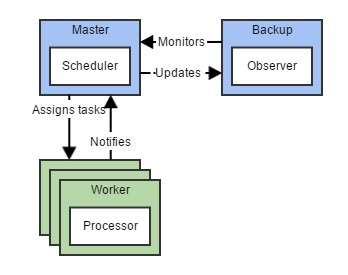
\includegraphics[width=0.4\textwidth]{images/architecture_overview.jpg}
	\caption{An overview of the system architecture on a high level. Multiple Workers are controlled by a Master node. The Backup node monitors the state of the Master node.}
	\label{fig:architecture_overview}
\end{figure}

\subsubsection{Master and Scheduler}
The Master node is the heart of the system, it receives new tasks and handles the scheduling.
The Master keeps a queue of all tasks that still need to be performed.
It assigns these tasks to Worker nodes and gets notified of finished tasks by the Workers.
The assignment of tasks is done by the Scheduler application.
Furthermore, the Scheduler instantiates new Worker nodes when the queue becomes too long.
These Worker nodes are stopped again when they have been inactive for a set period of time.
The scheduling policy will be further addressed in Section \ref{sec:policies}.

\subsubsection{Backup}
The Backup node monitors the state of the Master node and receives updates on new and finished tasks.
Incoming images are also send to the Backup node, so that they are available when the Master goes down.
The Backup node takes over the Masters work when the Master node becomes unavailable.

\subsubsection{Worker}
Worker nodes perform the actual work, they blur the image by applying a Gaussian filter.
These nodes receive tasks from the Master node, process them, and reply to the Master whenever a task is finished.
Worker nodes do not manage their own queue, they process one task at a time.

\subsubsection{Communication}
% TODO: Maria describe the communication between nodes

% a. Resource Management Architecture: describe the design of your system,
% including the inter-operation of the provisioning, allocation, reliability, and
% monitoring components (which correspond to the homonym features required
% by the WantCloud CTO).
\subsection{Resource Management Architecture}
\label{sec:resource_man}
This section will discuss how the designed architecture manages the resources of the cloud infrastructure.
Management of these resources is done according to the requirements given in Section \ref{sec:bg}.

\subsubsection{Elasticity}
The Scheduler, as discussed previously, manages the provisioning of Worker nodes as needed.
As the workload increases, the queue in the Master node builds up.
At a predetermined queue length, new Worker nodes will be provisioned.
These nodes are monitored by the Scheduler and stopped after a set period of inactivity.
The exact provisioning policy will be discussed in Section \ref{sec:policies}.

\subsubsection{Load Balancing}
The Scheduler balances the load by assigning tasks to the first available Worker node.
It does so by keeping track of all nodes and their states.
The four states a Worker node can be in are: Stopped, Starting, Idle, and Working.
As the names suggest, they imply that the node is turned off, starting up, waiting for work or processing a task respectively.
An Idle node is ready to receive a new task, it is therefore preferred as a node to assign tasks to.
If no Idle node can be found, the Scheduler either waits for a node to become Idle or provisions a new one, depending on the length of the queue.

\subsubsection{Reliability}
To ensure reliability, two monitoring features have been built into the design.
The first is the Master monitoring the Workers.
If a Worker node does not finish a tasks within a given period of time, it is assumed that the node crashed and it is shut down.
The task that Worker was working on will then be reintroduced to the queue and assigned to the next available node.

The second monitoring feature is the Backup node.
This node receives all uploaded images from the Master as well as all incoming connections from Worker nodes.
If no message can be sent, the Master notifies the Backup that it is still alive.
This way the Backup node knows if the Master is still working properly.
When there is no communication for a given period of time, the Backup node takes over and notifies all Workers that it has become the Master node.
Furthermore, the Master node is rebooted and initiated as the Backup node.

\subsubsection{Monitoring}
To monitor all the work that is being done in the system, logs are kept.
These logs are written to files on each server, keeping track of its own work.
The Master node logs the assignment and completion of tasks.
Worker nodes log incoming tasks, their processing and their completion.
These logs give an insight in processing times and load on each node.

% b. System Policies: describe the policies your system uses and supports. The latter
% may remain not implemented throughout your coursework, as long as you can
% explain how they can be supported in the future.
\subsection{System Policies}
\label{sec:policies}
As mentioned in several previous sections, specific functions of the system are controlled through policies.
Especially the work of the Scheduler depends very much on these set policies.
The following subsections will discuss the use of these policies, their current settings, and the possibility to extend this using custom policies.

\subsubsection{Scheduling}
Scheduling, consisting of load balancing and provisioning, is the core of the designed system.
It is used to assign tasks to available nodes, making optimal use of resources.
The Scheduler component has several settings that help it perform best, mostly related to the provisioning of new nodes.
The system stores these settings in a properties file, they are summed up in Table \ref{tbl:policy}.

\begin{table}
	\centering
	\begin{tabular}{| l | l | r |}
		\hline
		Setting name & Description & Value \\ \hline \hline
		\texttt{interval} & Scheduler interval & 2 sec. \\ \hline
		\texttt{loadThresh} & Max. tasks in queue & 5/node \\ \hline
		\texttt{maxTaskTime} & Max. time a Worker is Working & 1 min. \\ \hline
		\texttt{maxIdleTime} & Max. time a Worker is Idle & 1 hour \\ \hline
		\texttt{maxTaskRetry} & Max. times a task is retried & 2 x\\ \hline
		\texttt{maxTimeOut} & Max. times Master is unresponsive & 10 sec. \\ \hline
	\end{tabular}
	\caption{Settings for the different policies. These values describe the behaviour of the scheduling and the reliability policies.}
	\label{tbl:policy}
\end{table}

The basic choice for the scheduler is to assign a new task to the first available Worker node.
When no Worker node is available the Scheduler checks the length of the queue with the given policy.
As seen in Table \ref{tbl:policy}, the value of \texttt{loadThresh} indicates that if more than 5 tasks per working node are in the queue, a new Worker node should be provisioned.
This number was chosen as processing 5 tasks generally takes longer than provisioning a new Worker.

When a Worker node has been Idle for an hour, as set by \texttt{maxIdleTime}, it is shut down.
This period was chosen because the system is run on the Amazon EC2 cloud, in which starting up a machine costs the equivalent of one hour of compute power.
Shutting down a machine sooner and provisioning it again multiple times within an hour would cause a tremendous increase in cost.

\subsubsection{Reliability}
The other settings in Table \ref{tbl:policy} are used for reliability of the system.
\texttt{maxTaskTime} is used to indicate after what period the Master can consider a Worker node to have crashed, in this case it is set to 1 minute.
However, it should be considered that this period should be substantially longer than the maximum length an actual (non-crashed) task might take.

\texttt{maxTaskRetry} is the maximum amount of times a task is reassigned after a Worker node crashed on it.
With these settings if two nodes fail on the same task, the task is considered corrupt and ignored for further processing.

\texttt{maxTimeOut} is the maximum period in which the Backup node has not been able to contact the Master node.
If this period has passed, the Backup node takes over as the Master node.
This period is set to 10 seconds, as the Master node should normally send a message to the Backup node every 2 seconds (the \texttt{interval} setting).

\subsubsection{Extensions}
As the implemented policies are stored in properties files, they can easily be replaced or edited.
This allows the designed system to support different policies as well as enables WantCloud to fine-tune the policies according to the monitoring results.
Flexibility added this way allows the system to be adapted to changes in the environment, or nature of the tasks it performs.

% 6. Experimental Results (recommended size: 1.5 pages)
% a. Experimental set-up: describe the working environments (DAS, Amazon EC2,
% etc.), the general workload and monitoring tools and libraries, other tools and
% libraries you have used to implement and deploy your system, other tools and
% libraries used to conduct your experiments.
\section{Evaluation}
\label{sec:eval}
To verify whether the designed system offers an improvement to WantCloud, experiments have been conducted.
These experiments analyse the performance of the system as well as analyse the previously described features.
This section will first discuss the experimental set-up, giving an overview of the used environment and the implementation of the proof of concept.
Following subsections will discuss the conducted experiments and their results.

\subsection{Experimental Set-up}
The working environment chosen for this system is Amazon Web Services\cite{web:aws}, particularly the Elastic Compute Cloud (EC2)\cite{web:ec2}.
Virtual machines called EC2 instances can easily be provisioned on this infrastructure.
Moreover, the platform offers many tools to create divers applications.

The chosen instances are \texttt{t2.micro} instances with an Ubuntu operating system.
This instance type only offer one virtual CPU and 1 gigabyte of memory.
However, these instances can be used free of charge for 750 hours per month, leaving enough space to perform the experiments at no cost.
Six of these instances were created, of which one functioned as Master node, one as Backup node and four as Worker nodes.

The implementation of the system was done in Java and applies several external tools to perform all its work.
The most notably are the Gaussian blur implementation by Huxtable \cite{web:huxtable} and the AWS SDK for Java \cite{web:sdk}.
The full implementation of the experimental set-up is available as open source through GitHub \cite{web:git}.

% b. Experiments: describe the experiments you have conducted to analyse each
% system feature, then analyse them; use one sub-section per experiment. For
% each experiment, describe the workload, present the operation of the system,
% and analyse the results. In the analysis, report:
% i. Charged-time = time that would have been charged using the
% Amazon EC2 timing approach (1-hour increments)
% ii. Charged-cost = cost that would have been charged using the
% Amazon EC2 charging approach, assuming 10 Euro-cents/charged hour
% iii. Service metrics of the experiment, such as runtime and response time of
% the service, etc.
% iv. (optional) Usage metrics of the experiment, such as per-VM and overall
% system usage and activity.
\subsection{Scheduler Performance}
The first conducted experiment tests the performance of several scheduler set-ups against the performance of the current WantCloud server.

\subsubsection{Test set}
To understand this experiment, it is important to first describe the test set that was used.
The total test set consists of 20 images, which are listed in Table \ref{tbl:tasks}.
The table shows the file name, their size in kilobytes, their occurrence in the test set (\#), and the average time it took to process that image over all tests.
This set consists of four different images, of different sizes representing typical images.
There are two occurrences of the rather large \emph{strawberry.jpg}, and more occurrences of the smaller images.
As can be expected, it is easier to compute a Gaussian filter for small images than it is for large images.

\begin{table}
	\centering
	\begin{tabular}{| l | r | c | r |}
		\hline
		File name & Size (kB) & \# & Avg. time (sec.) \\ \hline \hline
		\emph{apple.jpeg} & 90.5 & 4 & 0.548 \\ \hline
		\emph{banana.jpg} & 342.2 & 7 & 17.312 \\ \hline
		\emph{pears.jpg} & 957.2 & 7 & 17.468 \\ \hline
		\emph{strawberry.jpg} & 5,735.9 & 2 & 26.226 \\ \hline
	\end{tabular}
	\caption{Selected set of test images, their size in kilobytes, their occurrence in the test set (total: 20 images), and their average processing time over all tests.}
	\label{tbl:tasks}
\end{table}

\subsubsection{Experiment}
In this experiment the current WantCloud approach is simulated by using a single EC2 instance that operates directly on input files, without the use of a scheduler.
The used set-ups are listed in Table \ref{tbl:setups}.
In this table, the \emph{Single} set-up is the instance just described.
The other set-ups use the Scheduler and have respectively one, two, three or four Worker nodes to perform the work. 

\begin{table}
	\centering
	\begin{tabular}{| l | c | c |}
		\hline
		Name & Scheduler & \# Worker \\ \hline \hline
		\emph{Single} & no & - \\ \hline
		\emph{Scheduler 1} & yes & 1 \\ \hline
		\emph{Scheduler 2} & yes & 2 \\ \hline
		\emph{Scheduler 3} & yes & 3 \\ \hline
		\emph{Scheduler 4} & yes & 4 \\ \hline
	\end{tabular}
	\caption{The different set-ups tested in the Scheduler Performance experiment, the name, use of the Scheduler, and amount of used Worker nodes are listed.}
	\label{tbl:setups}
\end{table}

\subsubsection{Results}
The results of this experiment are shown in Figure \ref{fig:diagram_total_processing}.
This figure shows the total processing time for the whole test set per set-up.
Several interesting facts stand out when analysing these results.
First of all it can be seen that \emph{Scheduler 1} takes a few seconds longer than \emph{Single}.
This is as expected, as the Scheduler would cause some overhead.
Interestingly, this overhead is quite minimal.

\begin{figure}
	\centering
	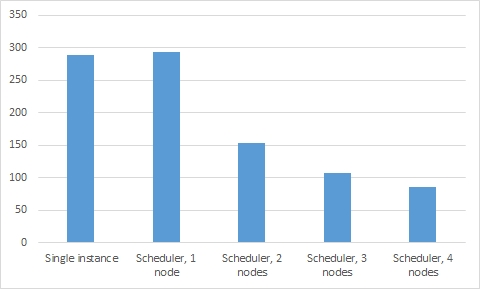
\includegraphics[width=0.5\textwidth]{images/diagram_total_processing.jpg}
	\caption{Processing time comparison for 5 types of set-ups. Time in seconds.}
	\label{fig:diagram_total_processing}
\end{figure}

The following observation that can be made is that \emph{Scheduler 2} scores significantly better than both previous set-ups.
The speed up is almost double compared to \emph{Scheduler 1}.
\emph{Scheduler 3} and \emph{Scheduler 4} both perform even better than the previous two.

To verify these results the average processing time per task was also analysed in Figure \ref{fig:diagram_avg_image}.
This figure shows that the average time per task is almost the same in each set-up.
A small increase can be seen from \emph{Single} to the \emph{Scheduler} set-ups, which could be due to the Scheduler overhead.
However, this difference is so small it is hardly measurable on this scale.

\begin{figure}
	\centering
	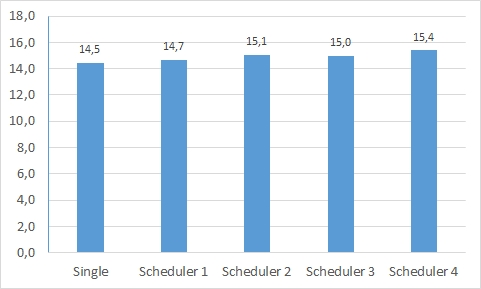
\includegraphics[width=0.5\textwidth]{images/diagram_avg_image.jpg}
	\caption{Average processing time per task for 5 types of set-ups. Time in seconds.}
	\label{fig:diagram_avg_image}
\end{figure}

Table \ref{tbl:costs} gives an overview of estimated costs using the different set-ups on Amazon EC2.
For \emph{Single} only one machine is needed, which keeps the cost low.
For \emph{Scheduler 1} to \emph{4}, not only the Worker node, but also a Master node and a Backup node are required, this results in higher costs per running hour.
As these tests were relatively brief, they do not predict the costs for long term use of the system.
In the long term, the \emph{Scheduler} set-ups require at least two machines to be running at all time (Master and Backup), Workers can be shut off.
Further discussion of these costs can be found in Section \ref{sec:discussion}.

\begin{table}
	\centering
	\begin{tabular}{| l | c | c |}
		\hline
		Name & EC2 hours & Costs (\euro) \\ \hline \hline
		\emph{Single} & 1 & 0,10 \\ \hline
		\emph{Scheduler 1} & 3 & 0,30 \\ \hline
		\emph{Scheduler 2} & 4 & 0,40 \\ \hline
		\emph{Scheduler 3} & 5 & 0,50 \\ \hline
		\emph{Scheduler 4} & 6 & 0,60 \\ \hline
	\end{tabular}
	\caption{The charged hours and costs of the different set-ups tested in the Scheduler Performance experiment, on Amazon EC2. Cost per hour: \EUR{0,10}.}
	\label{tbl:costs}
\end{table}

\subsection{Time To Recover Master}

\subsubsection{Experiment}

\subsubsection{Results}

\subsection{Time To Boot}

\subsubsection{Experiment}

\subsubsection{Results}

% 7. Discussion (recommended size: 1 page): summarize the main findings of your work
% and discuss the tradeoffs inherent in the design of cloud-computing-based applications.
% Should the WantCloud CTO use IaaS-based clouds? Among others, use extrapolation
% on the results, as reported in Section 6.b of the report, to discuss the charged time and
% charged cost reported in section for 100,000/1,000,000/10,000,000 users and for 1
% day/1 month/1 year.
\section{Discussion}
\label{sec:discussion}

% 8. Conclusion
\section{Conclusion}
\label{sec:conclusion}

\bibliography{references}{}
\bibliographystyle{plain}

\appendix
% 9. Appendix A: Time sheets (see Section E)
\section{Time sheet}

The following table documents the time spent working on specific parts of the assignment.

\begin{tabular}{ | l | r | }
	\hline
	Part & Time (hrs) \\ \hline \hline
	% the  = total amount of time spent in completing WantOne CTO’s assignment (the large exercise).
	\texttt{total-time} & 50\\ \hline
	% the think-time = total amount of time spent in thinking about how to solve WantOne CTO’s assignment (the large exercise).
	\texttt{think-time} & 8\\ \hline
	% the dev-time = total amount of time spent in developing the code needed to solve WantOne CTO’s assignment (the large exercise).
	\texttt{dev-time} & 40\\ \hline
	% the xp-time = total amount of time spent in experiments for WantOne CTO’s assignment (the large exercise).
	\texttt{xp-time} & 0\\ \hline
	% the analysis-time = total amount of time spent in analyzing the results of the experiments for WantOne CTO’s assignment (the large exercise).
	\texttt{analysis-time} & 0\\ \hline
	% the write-time = total amount of time spent in writing this report
	\texttt{write-time} & 2\\ \hline
	% the wasted-time = total amount of time spent in activities related to WantOne CTO’s assignment (the large exercise), but which cannot be charged as think-time, dev-time, xp-time, analysis-time, or write-time
	\texttt{wasted-time} & 0\\ \hline
\end{tabular}

\end{document}